\chapter{Phương pháp nghiên cứu và giải pháp đề xuất}
\label{chap:method-solution}

Chương này trình bày phương pháp nghiên cứu và giải pháp đề xuất cho bài toán tối ưu bộ luật WAF ModSecurity trong phát hiện Cross-Site Scripting và SQL Injection. Nếu Chương 2 xây dựng nền tảng về WAF, ModSecurity, OWASP CRS, XSS, SQLi và các hướng phát hiện liên quan, thì chương này mô tả cách khóa luận tiếp cận bài toán và thiết kế bộ generalized rules v2. Nội dung bắt đầu từ quy trình nghiên cứu tổng thể, sau đó trình bày nguyên tắc phương pháp luận, kiến trúc giải pháp, thiết kế XSS/SQLi rules, decode pipeline, tích hợp anomaly scoring và phương pháp tuning.

Chương này không đi sâu vào môi trường chạy thí nghiệm, dataset hay công cụ benchmark. Các nội dung đó được trình bày ở Chương 4 sau khi giải pháp đã được mô tả đầy đủ. Cách sắp xếp này giúp mạch luận văn đi từ vấn đề và phương pháp đề xuất tới thiết kế đánh giá, phù hợp hơn với cấu trúc của một bài báo khoa học hoặc đồ án kỹ thuật.

\section{Tổng quan quy trình nghiên cứu}
\label{sec:research-workflow}

Quy trình nghiên cứu của khóa luận được xây dựng theo hướng lặp: phân tích hệ thống hiện có, thiết kế cải tiến, đánh giá định lượng, phân tích lỗi và tiếp tục tuning. Cách tiếp cận này phù hợp với bài toán tối ưu WAF vì chất lượng của rule không thể được đánh giá chỉ bằng cách đọc regex. Một rule có thể hợp lý ở mức cú pháp nhưng vẫn bỏ sót payload bị mã hóa, hoặc chặn nhầm nhiều request hợp lệ khi chạy trên dữ liệu thực tế. Do đó, mỗi thay đổi trong rule cần được kiểm chứng bằng benchmark và audit log~\cite{benchmark-methodology,waf-tuning-methodology}.

Hình~\ref{fig:research-pipeline-flow} mô tả luồng nghiên cứu tổng quát. Quy trình bắt đầu từ việc khảo sát OWASP CRS và các rule gốc theo hướng enumeration-based. Từ đó, các false negative và false positive được phân tích để xác định hạn chế của cách phát hiện dựa trên danh sách cố định. Tiếp theo, khóa luận thiết kế bộ generalized rules v2 cho XSS và SQLi, tích hợp rule với anomaly scoring của CRS, xây dựng phương pháp tuning dựa trên dữ liệu và cuối cùng thiết kế thực nghiệm để đánh giá giải pháp.

\begin{figure}[p]
    \centering
    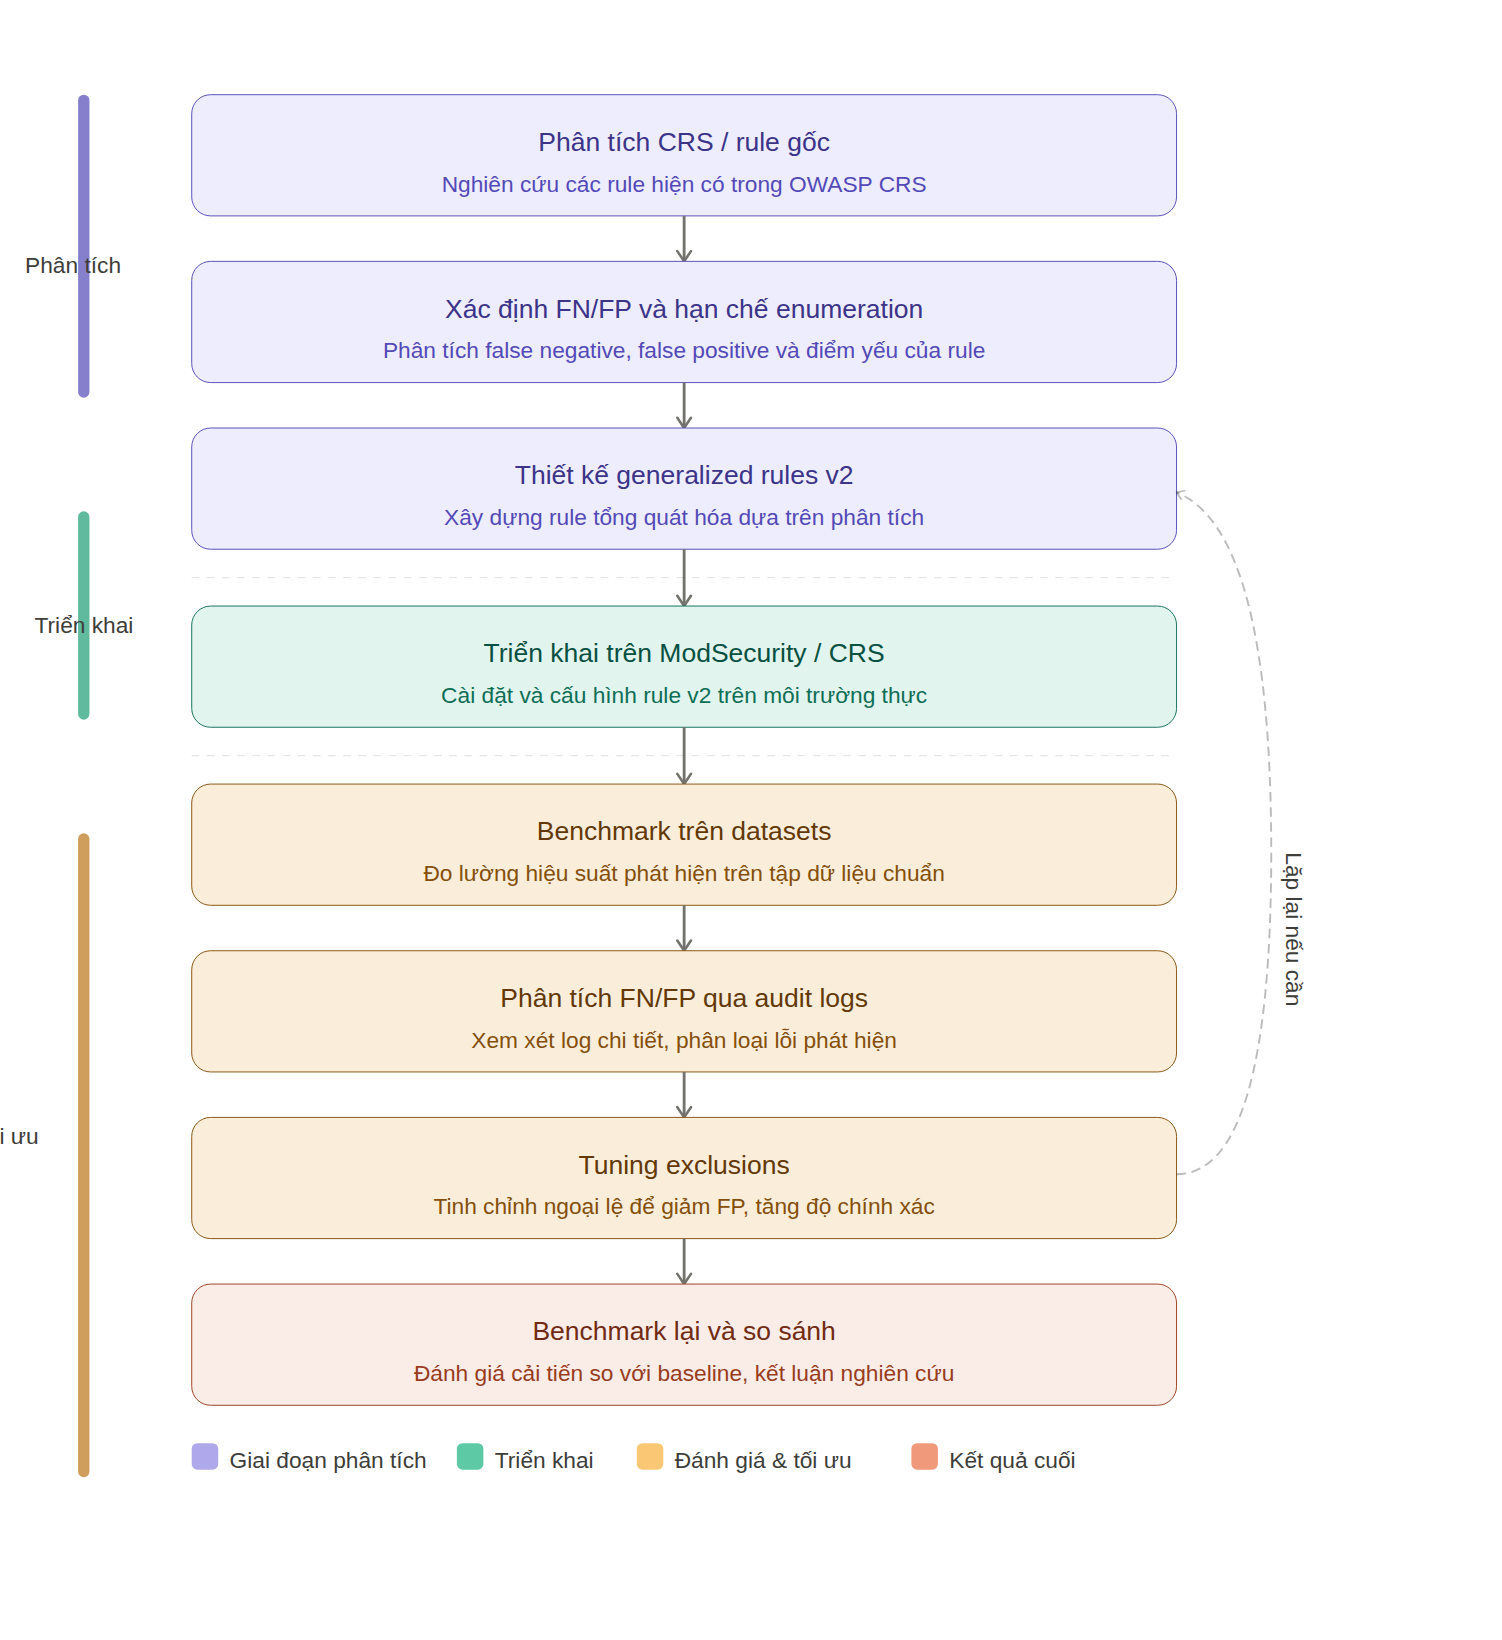
\includegraphics[width=0.92\textwidth,height=0.80\textheight,keepaspectratio]{Chapter3/research_pipeline_flow.png}
    \caption{Quy trình nghiên cứu tổng quát của khóa luận}
    \label{fig:research-pipeline-flow}
\end{figure}

Có thể chia quy trình trên thành ba giai đoạn chính. Giai đoạn thứ nhất là phân tích, bao gồm tìm hiểu CRS, rule gốc và các nhóm payload gây lỗi. Giai đoạn thứ hai là đề xuất giải pháp, bao gồm thiết kế rule v2, decode pipeline, anomaly scoring integration và tuning methodology. Giai đoạn thứ ba là đánh giá, bao gồm thiết kế môi trường thực nghiệm, chạy benchmark, phân tích FN/FP và so sánh với baseline. Chương này tập trung vào hai giai đoạn đầu; Chương 4 trình bày chi tiết giai đoạn đánh giá.

\section{Nguyên tắc phương pháp luận}
\label{sec:methodological-principles}

Phương pháp nghiên cứu của khóa luận dựa trên bốn nguyên tắc chính.

Thứ nhất, việc tối ưu WAF phải dựa trên dữ liệu thay vì chỉ dựa trên trực giác viết rule. Các false negatives cho biết rule còn bỏ sót kỹ thuật nào; các false positives cho biết rule nào quá rộng hoặc không phù hợp với traffic mục tiêu. Vì vậy, benchmark và audit log không chỉ được dùng để báo cáo kết quả cuối cùng, mà còn là công cụ để cải thiện rule theo vòng lặp.

Thứ hai, khóa luận ưu tiên generalized/context-aware detection thay vì enumeration-based detection. Với XSS, rule cần phát hiện ngữ cảnh thực thi như thẻ có khả năng chạy mã, event handler có giá trị nguy hiểm, protocol URI hoặc DOM sink. Với SQLi, rule cần phát hiện semantic patterns như \path|UNION SELECT|, stacked query, boolean bypass, time-based function hoặc schema enumeration. Cách tiếp cận này nhằm giảm phụ thuộc vào danh sách payload cố định.

Thứ ba, mục tiêu đánh giá không chỉ là tối đa hóa recall. Trong WAF, false positive rate có ý nghĩa vận hành rất lớn: một hệ thống chặn được nhiều payload tấn công nhưng đồng thời chặn nhầm nhiều request hợp lệ sẽ khó triển khai thực tế. Do đó, mọi cải tiến rule cần được đọc đồng thời qua recall, FPR, precision và các ví dụ FP/FN cụ thể.

Thứ tư, tuning CRS phải có kiểm soát. Việc dùng \path|SecRuleRemoveById| không được hiểu là tắt rule để làm đẹp chỉ số, mà là thay thế hoặc loại bỏ có chọn lọc các rule gây FP cao, trùng lặp với custom rules hoặc nằm ngoài phạm vi đánh giá. Mỗi quyết định tuning cần đi kèm bằng chứng từ benchmark, audit log và phân tích rủi ro.

\section{Kiến trúc tổng quan giải pháp}
\label{sec:solution-architecture}

Giải pháp được xây dựng trên kiến trúc WAF sử dụng ModSecurity kết hợp OWASP Core Rule Set. ModSecurity đóng vai trò WAF engine xử lý HTTP transaction, còn CRS cung cấp rule set nền, cơ chế anomaly scoring và rule chặn tổng hợp. Custom rules v2 được bổ sung vào cùng pipeline xử lý của CRS, thay vì hoạt động như một bộ lọc độc lập. Khi một rule v2 khớp với request, rule không chỉ ghi nhận dấu hiệu XSS/SQLi riêng mà còn cộng điểm vào biến inbound anomaly score của CRS. Quyết định cuối cùng Block/Pass vẫn dựa trên cơ chế threshold của CRS~\cite{modsecurity-docs,owasp-crs-docs,modsecurity-crs-overview}.

Hình~\ref{fig:modsecurity-architecture-flow} mô tả luồng xử lý tổng quát của giải pháp. HTTP request đi qua các phase của ModSecurity, được chuẩn hóa bởi các transformation cần thiết, sau đó được kiểm tra bởi hai nhóm custom rules chính: XSS generalized rules trong dải \path|9942xxx| và SQLi generalized rules trong dải \path|9943xxx|. Các rule này cộng điểm vào anomaly score tương ứng; sau đó CRS scoring engine, đặc biệt nhóm rule \path|949xxx|, đánh giá tổng điểm và quyết định request có bị chặn hay không.

\begin{figure}[p]
    \centering
    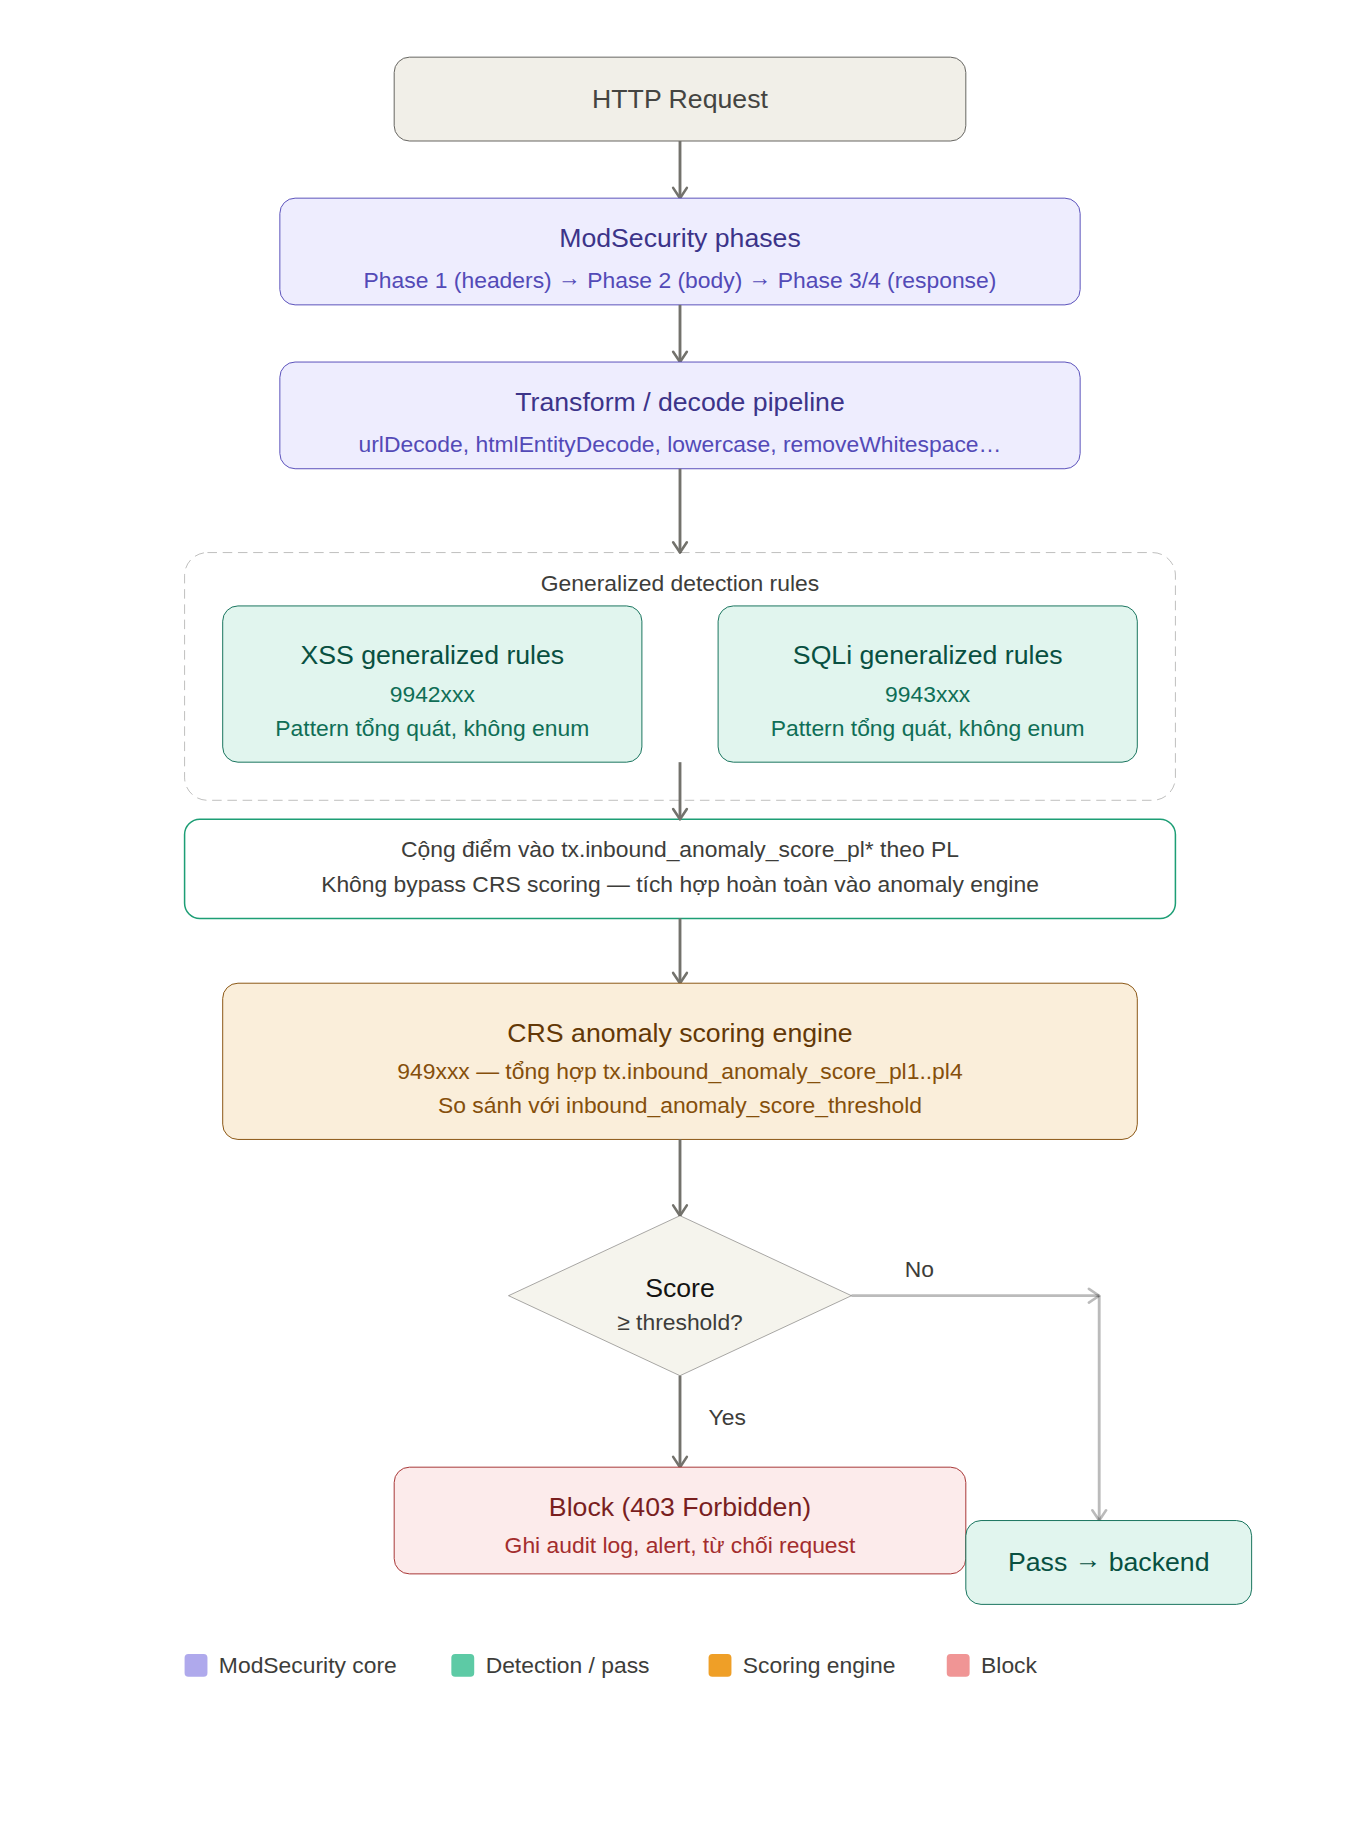
\includegraphics[width=0.92\textwidth,height=0.80\textheight,keepaspectratio]{Chapter4/modsecurity_architecture_flow.png}
    \caption{Kiến trúc xử lý request của giải pháp ModSecurity/CRS với generalized rules}
    \label{fig:modsecurity-architecture-flow}
\end{figure}

Bảng~\ref{tab:solution-logical-components} tóm tắt các thành phần logic trong giải pháp. Các chi tiết triển khai cụ thể như Docker image, backend thử nghiệm, tham số môi trường và audit log path được trình bày ở Chương 4 trong phần thiết kế thực nghiệm.

{\small
\renewcommand{\arraystretch}{1.2}
\begin{longtable}{|L{0.24\textwidth}|L{0.32\textwidth}|L{0.34\textwidth}|}
\caption{Các thành phần logic trong kiến trúc giải pháp}\label{tab:solution-logical-components}\\
\hline
\textbf{Thành phần} & \textbf{Vai trò} & \textbf{Ghi chú thiết kế} \\
\hline
\endfirsthead

\hline
\textbf{Thành phần} & \textbf{Vai trò} & \textbf{Ghi chú thiết kế} \\
\hline
\endhead

OWASP CRS nền & Cung cấp rule set tổng quát, anomaly scoring và rule đánh giá tổng điểm. & Không bị thay thế hoàn toàn; giải pháp chỉ chuyên biệt hóa phát hiện XSS/SQLi. \\
\hline
XSS generalized rules v2 & Phát hiện XSS theo hướng context-aware. & Dải ID \path|9942xxx|, tập trung vào execution context và payload encoded/obfuscated. \\
\hline
SQLi generalized rules v2 & Phát hiện SQLi theo hướng semantic-based. & Dải ID \path|9943xxx|, tập trung vào cấu trúc injection và coverage đa DBMS. \\
\hline
Decode pipeline & Chuẩn hóa payload trước khi so khớp. & Dùng URL decode, HTML entity decode, JavaScript decode, remove nulls, compress whitespace và Base64 decode có điều kiện. \\
\hline
Anomaly scoring integration & Cộng điểm vào CRS để quyết định block/pass theo threshold. & Rule v2 dùng severity khác nhau thay vì chặn mọi dấu hiệu với cùng mức độ. \\
\hline
Tuning exclusions & Giảm FP từ các CRS rules quá tổng quát hoặc trùng logic. & Được sử dụng có kiểm soát, dựa trên audit log và phân tích rủi ro. \\
\hline
\end{longtable}
}

Điểm quan trọng của kiến trúc này là custom rules v2 không thay thế toàn bộ CRS. Chúng được thiết kế để bổ sung và chuyên biệt hóa khả năng phát hiện XSS/SQLi, đồng thời tận dụng cơ chế scoring sẵn có của CRS. Việc tuning exclusions chỉ được áp dụng có chọn lọc trong phạm vi nghiên cứu để giảm nhiễu và giảm false positives, không phải khuyến nghị cấu hình mặc định cho mọi hệ thống production.

\section{Nguyên tắc thiết kế bộ luật v2}
\label{sec:rule-design-principles}

Bộ luật v2 được thiết kế theo hướng generalized thay vì enumeration-based. Cách tiếp cận enumeration-based thường mở rộng danh sách payload, từ khóa hoặc hàm đã biết. Cách này dễ triển khai ban đầu nhưng khó bao phủ các biến thể mới và dễ gây false positives khi pattern quá rộng. Ngược lại, generalized rules cố gắng mô tả cấu trúc hoặc ngữ cảnh tấn công ở mức tổng quát hơn: XSS được nhìn dưới góc độ execution context, còn SQLi được nhìn dưới góc độ semantic pattern của câu lệnh SQL bị chèn.

Nguyên tắc đầu tiên là context-aware detection cho XSS. Một chuỗi như \path|script|, \path|alert| hoặc \path|onload| không luôn là tấn công. Nó có thể xuất hiện trong tài liệu kỹ thuật, nội dung bài viết hoặc dữ liệu hợp lệ. Vì vậy, rule XSS v2 không chỉ kiểm tra sự tồn tại của từ khóa mà còn kiểm tra vị trí và ngữ cảnh thực thi, ví dụ thẻ \path|<script>| có nội dung thực thi, event handler có giá trị nguy hiểm, protocol URI \path|javascript:|, hoặc DOM sink như \path|innerHTML| đi kèm HTML/script injection.

Nguyên tắc thứ hai là semantic-based detection cho SQLi. SQLi v2 không bắt các keyword rời như \path|select| hoặc \path|or| một cách độc lập, vì các từ này có thể xuất hiện trong dữ liệu hợp lệ. Thay vào đó, rule tập trung vào các cấu trúc có ý nghĩa injection, chẳng hạn \path|UNION SELECT|, stacked query bắt đầu bằng dấu chấm phẩy và theo sau là DML/DDL keyword, quote kết hợp toán tử logic và tautology, hàm time-based blind SQLi hoặc truy cập system catalog.

Nguyên tắc thứ ba là chuẩn hóa dữ liệu trước khi so khớp. Payload tấn công có thể được URL encode, HTML entity encode, JavaScript escape, chèn null byte hoặc chèn khoảng trắng bất thường. Vì vậy, nhiều rule v2 sử dụng các transformation như \path|t:urlDecodeUni|, \path|t:htmlEntityDecode|, \path|t:jsDecode|, \path|t:removeNulls| và \path|t:compressWhitespace| trước khi áp dụng regex. Với Base64, giải pháp dùng các rule chuyên biệt để decode rồi kiểm tra lại nội dung đã decode, thay vì coi mọi chuỗi Base64 là tấn công.

Nguyên tắc thứ tư là hiệu chỉnh severity theo độ tin cậy của dấu hiệu. Các pattern có độ tin cậy cao như \path|UNION SELECT|, event handler gọi hàm nguy hiểm hoặc protocol URI \path|javascript:| được gán mức \path|CRITICAL|. Các pattern encoded/obfuscated hoặc error-based có thể gán \path|ERROR|. Các pattern context-specific hoặc heuristic nâng cao có thể gán \path|WARNING| hoặc \path|NOTICE|. Cách phân tầng này giúp rule v2 hòa vào anomaly scoring thay vì chặn mọi dấu hiệu với cùng mức nghiêm trọng.

Nguyên tắc cuối cùng là giảm false positives bằng cách giới hạn phạm vi input target và tổ chức rule dễ bảo trì. XSS v2 cố ý không scan \path|REQUEST_HEADERS:User-Agent| vì header này thường chứa chuỗi phức tạp từ trình duyệt, bot hoặc công cụ tự động, dễ gây FP nếu kiểm tra quá rộng. Các rule được chia theo dải ID và lớp kỹ thuật, giúp khi xuất hiện bypass mới có thể thêm rule vào đúng lớp thay vì nối thêm payload vào một regex lớn khó kiểm soát.

\section{Thiết kế XSS generalized rules v2}
\label{sec:xss-rules-v2}

Bộ XSS generalized rules v2 được triển khai trong file \path|REQUEST-941-XSS-GENERALIZED-v2.conf| với dải ID \path|9942000-9942074|. Rule \path|9942000| là rule khởi tạo, đặt biến \path|tx.xss_score_v2| về 0 ở đầu quá trình xử lý. Các rule còn lại phát hiện những nhóm XSS khác nhau và cộng điểm vào cả biến riêng \path|tx.xss_score_v2| lẫn biến \path|tx.inbound_anomaly_score_pl*| của CRS.

Tư tưởng chính của XSS v2 là phát hiện dựa trên ngữ cảnh thực thi. Thay vì chặn mọi HTML tag hoặc mọi event handler, rule cố gắng xác định khi nào dữ liệu đầu vào có khả năng tạo execution context trong trình duyệt. Bảng~\ref{tab:xss-v2-layers} tóm tắt các lớp chính của XSS v2.

{\small
\setlength{\tabcolsep}{4pt}
\renewcommand{\arraystretch}{1.25}
\begin{longtable}{|L{0.17\textwidth}|C{0.15\textwidth}|C{0.13\textwidth}|L{0.43\textwidth}|}
\caption{Các lớp phát hiện trong XSS generalized rules v2}\label{tab:xss-v2-layers}\\
\hline
\textbf{Lớp} & \textbf{Rule ID} & \textbf{Severity} & \textbf{Mục tiêu và kỹ thuật tiêu biểu} \\
\hline
\endfirsthead

\hline
\textbf{Lớp} & \textbf{Rule ID} & \textbf{Severity} & \textbf{Mục tiêu và kỹ thuật tiêu biểu} \\
\hline
\endhead

L1 Core XSS & \makecell{\texttt{9942001}\\--\\\texttt{9942004}} & \texttt{CRITICAL} & Phát hiện các ngữ cảnh XSS trực tiếp, có độ tin cậy cao, ví dụ \path|<script>| có execution, \path|onerror=alert| và protocol URI \path|javascript:|. \\
\hline
L2 Structural injection & \makecell{\texttt{9942010}\\--\\\texttt{9942013}} & \texttt{CRITICAL} & Phát hiện cấu trúc HTML/SVG/CSS có khả năng kích hoạt mã, gồm SVG event, iframe/object có nguồn nguy hiểm, CSS execution và executable \path|data:| URI. \\
\hline
L3 Encoded/obfuscated & \makecell{\texttt{9942020}\\--\\\texttt{9942025}} & \texttt{ERROR} & Phát hiện payload bị mã hóa hoặc chia nhỏ để né regex trực tiếp, gồm double URL encode, HTML entity, Base64 decode-and-check và string concatenation. \\
\hline
L4 DOM context & \makecell{\texttt{9942030}\\--\\\texttt{9942032}} & \texttt{WARNING} & Phát hiện DOM-based XSS và cách gọi hàm gián tiếp, ví dụ \path|innerHTML|, \path|document.write|, bracket notation và template literal. \\
\hline
L5 Advanced/heuristic & \makecell{\texttt{9942040}\\--\\\texttt{9942074}} & \makecell{\texttt{NOTICE}\\--\\\texttt{CRITICAL}} & Phát hiện các kỹ thuật bypass nâng cao và lớp Base64 chuyên biệt, gồm prototype chain, optional chaining, array callback, function alias và tag splitting. \\
\hline
\end{longtable}
}

\subsection{Lớp 1: Core XSS}
\label{subsec:xss-core-layer}

Lớp 1 tập trung vào các dấu hiệu XSS trực tiếp và có độ tin cậy cao. Rule \path|9942001| phát hiện thẻ \path|<script>| khi bên trong có execution context như \path|alert|, \path|eval|, \path|document.cookie|, \path|location| hoặc các thao tác DOM nguy hiểm. Điểm quan trọng là rule không chỉ bắt sự xuất hiện của chuỗi \path|<script>|, vì một thẻ script tham chiếu tài nguyên hợp lệ có thể xuất hiện trong dữ liệu benign.

Rule \path|9942002| phát hiện event handler có giá trị nguy hiểm. Một thuộc tính như \path|onsubmit| không tự động bị xem là XSS; rule chỉ có ý nghĩa khi phần giá trị sau dấu bằng gọi hàm hoặc đối tượng nguy hiểm, chẳng hạn \path|alert|, \path|eval|, \path|document.|, \path|window.|, \path|Function| hoặc \path|setTimeout|. Cách này thể hiện rõ nguyên tắc context-aware: cùng là event handler, nhưng giá trị thực thi quyết định mức rủi ro.

Rule \path|9942003| phát hiện protocol URI như \path|javascript:| hoặc \path|vbscript:|, kể cả khi chuỗi bị chèn khoảng trắng hoặc ký tự điều khiển giữa các chữ cái. Rule \path|9942004| phát hiện các dangerous JavaScript function calls và thao tác nguy hiểm như truy cập cookie hoặc gán vào location. Các rule lớp 1 đều có severity \path|CRITICAL| và cộng điểm vào \path|tx.inbound_anomaly_score_pl1|, vì đây là các tín hiệu có độ tin cậy cao.

\subsection{Lớp 2: Structural injection}
\label{subsec:xss-structural-layer}

Lớp 2 xử lý các cấu trúc HTML hoặc browser feature có thể tạo execution context mà không nhất thiết dùng trực tiếp thẻ \path|<script>|. Rule \path|9942010| tập trung vào các thẻ như SVG, MathML, media tag hoặc các cấu trúc tương tự khi đi kèm event handler. Đây là nhóm quan trọng vì nhiều payload XSS sử dụng \path|<svg onload=...>| hoặc các biến thể tương tự để kích hoạt JavaScript.

Rule \path|9942011| phát hiện các thẻ nhúng nội dung bên ngoài như \path|iframe|, \path|object|, \path|embed| hoặc \path|applet| khi thuộc tính nguồn có dấu hiệu đáng ngờ như \path|javascript:| hoặc \path|data:|. Rule \path|9942012| phát hiện style injection có execution context, ví dụ \path|expression()|, \path|behavior:| hoặc URL trong CSS trỏ tới \path|javascript:|. Rule \path|9942013| phát hiện \path|data:| URI với MIME có thể thực thi như \path|text/html| hoặc JavaScript.

Các rule structural injection cũng được gán \path|CRITICAL|, nhưng được cộng vào \path|tx.inbound_anomaly_score_pl2|. Việc tách lớp giúp phân biệt giữa core XSS trực tiếp và các cấu trúc HTML/CSS/SVG nguy hiểm, đồng thời giúp audit log dễ truy vết nguyên nhân hơn.

\subsection{Lớp 3: Encoded và obfuscated XSS}
\label{subsec:xss-encoded-layer}

Lớp 3 xử lý payload đã bị mã hóa hoặc biến đổi để né rule đơn giản. Rule \path|9942020| phát hiện double/triple URL encoding, ví dụ các dạng biểu diễn của dấu nhỏ hơn hoặc thẻ HTML bị mã hóa nhiều lớp. Với những payload như vậy, nếu WAF chỉ decode một lần hoặc không kiểm tra dạng encoded nguyên bản, payload có thể đi qua và chỉ trở thành mã nguy hiểm ở phía ứng dụng.

Rule \path|9942021| phát hiện HTML entity bypass, chẳng hạn \path|&lt;script| hoặc các entity biểu diễn dấu hai chấm, dấu ngoặc và ký tự liên quan tới JavaScript. Rule \path|9942024| nhắm tới string concatenation bypass, nơi tên hàm hoặc chuỗi nguy hiểm được chia nhỏ rồi nối lại ở runtime. Các kỹ thuật này cho thấy XSS không chỉ xuất hiện dưới dạng chuỗi rõ ràng, mà có thể được biểu diễn bằng nhiều lớp ngữ pháp khác nhau của HTML và JavaScript.

Một điểm đáng chú ý trong lớp 3 là chuỗi rule \path|9942022-9942025| cho Base64. Rule đầu tiên bắt candidate có dạng Base64, rule tiếp theo decode và lưu vào biến \path|TX|, sau đó rule kiểm tra nội dung đã decode có chứa XSS execution context hay không. Thiết kế này tránh việc chặn mọi chuỗi Base64, đồng thời vẫn phát hiện được payload bị giấu trong lớp mã hóa. Các rule lớp 3 thường có severity \path|ERROR| và cộng vào \path|tx.inbound_anomaly_score_pl3|.

\subsection{Lớp 4: DOM context}
\label{subsec:xss-dom-layer}

Lớp 4 tập trung vào DOM-based XSS và các cách gọi hàm gián tiếp trong JavaScript. Rule \path|9942030| phát hiện thao tác DOM như \path|innerHTML|, \path|outerHTML|, \path|document.write| hoặc các sink tương tự khi đi kèm nội dung HTML/script nguy hiểm. Đây là nhóm quan trọng vì DOM-based XSS thường không chỉ dựa vào thẻ HTML, mà dựa vào việc JavaScript phía client ghi dữ liệu không tin cậy vào DOM.

Rule \path|9942031| phát hiện bracket notation execution, ví dụ \path|window['alert']| hoặc các biến thể gọi hàm thông qua tên chuỗi. Kỹ thuật này thường được dùng để né regex chỉ bắt lời gọi hàm trực tiếp. Rule \path|9942032| phát hiện template literal hoặc cú pháp gọi hàm đặc thù của JavaScript hiện đại. Các rule lớp 4 được gán \path|WARNING| vì chúng mang tính context-specific hơn, có thể cần kết hợp với các tín hiệu khác trong anomaly scoring.

\subsection{Lớp 5: Advanced heuristic và Base64 dedicated layer}
\label{subsec:xss-advanced-layer}

Lớp 5 bao gồm các kỹ thuật bypass nâng cao, với severity thay đổi từ \path|NOTICE| đến \path|CRITICAL| tùy mức độ nguy hiểm của pattern. Rule \path|9942040| xử lý prototype chain exploitation; rule \path|9942041| phát hiện advanced function reference như gọi hàm qua \path|call|, đặt hàm trong ngoặc hoặc dùng cú pháp ít phổ biến. Rule \path|9942057| phát hiện JS context break-out, tức payload cố thoát khỏi chuỗi hoặc ngữ cảnh JavaScript hiện có để chèn lệnh mới.

Một số rule khác trong lớp này xử lý array callback XSS, variable assignment/function alias, named entity bypass, custom tag kết hợp event handler, optional chaining và double angle bracket. Rule \path|9942074| nhắm tới tag-splitting evasion, khi payload chia nhỏ token nguy hiểm bằng thẻ hoặc ký tự xen giữa để làm regex trực tiếp không khớp. Các rule này không nhất thiết cùng một mức severity vì độ tin cậy của từng pattern khác nhau.

Ngoài chuỗi Base64 trong lớp 3, XSS v2 còn có dedicated Base64 layer ở dải \path|9942070-9942074|. Lớp này áp dụng \path|t:base64Decode| có chủ đích, sau đó kiểm tra lại nội dung đã decode bằng các pattern XSS. Vai trò của lớp này là tăng khả năng phát hiện payload bị đóng gói trong Base64, đặc biệt trong các benchmark evasion. Tuy nhiên, Base64 decode vẫn cần được xem như lớp bổ sung, không phải bằng chứng tấn công nếu không có execution context sau decode.

Thiết kế XSS v2 là cơ sở kỹ thuật để trả lời RQ1 và RQ2. RQ1 được kiểm chứng bằng việc so sánh false positives của context-aware rules với enumeration-based rules; RQ2 được kiểm chứng bằng các payload encoded/obfuscated và các false negatives còn lại sau benchmark.

\section{Thiết kế SQLi generalized rules v2}
\label{sec:sqli-rules-v2}

Bộ SQLi generalized rules v2 được triển khai trong file \path|REQUEST-942-SQLI-GENERALIZED-v2.conf| với dải ID \path|9943000-9943043|. Rule \path|9943000| khởi tạo biến \path|tx.sqli_score_v2|. Các rule còn lại phát hiện SQL Injection theo hướng semantic-based, tức tập trung vào cấu trúc injection và hành vi truy vấn hơn là bắt keyword rời.

SQLi v2 bao phủ nhiều nhóm kỹ thuật phổ biến trên nhiều hệ quản trị cơ sở dữ liệu. Một số rule nhắm tới cú pháp chung như \path|UNION SELECT| hoặc stacked query; một số rule nhắm tới hàm đặc thù như \path|sleep|, \path|waitfor delay|, \path|pg_sleep|, \path|extractvalue| hoặc \path|xp_dirtree|. Bảng~\ref{tab:sqli-v2-layers} tóm tắt các lớp chính của SQLi v2.

{\small
\setlength{\tabcolsep}{4pt}
\renewcommand{\arraystretch}{1.25}
\begin{longtable}{|L{0.17\textwidth}|C{0.15\textwidth}|C{0.13\textwidth}|L{0.43\textwidth}|}
\caption{Các lớp phát hiện trong SQLi generalized rules v2}\label{tab:sqli-v2-layers}\\
\hline
\textbf{Lớp} & \textbf{Rule ID} & \textbf{Severity} & \textbf{Mục tiêu và kỹ thuật tiêu biểu} \\
\hline
\endfirsthead

\hline
\textbf{Lớp} & \textbf{Rule ID} & \textbf{Severity} & \textbf{Mục tiêu và kỹ thuật tiêu biểu} \\
\hline
\endhead

L1 Classic SQLi & \makecell{\texttt{9943001}\\--\\\texttt{9943003}} & \texttt{CRITICAL} & Phát hiện các cấu trúc SQLi trực tiếp, thường gặp, gồm \path|UNION SELECT|, stacked query và boolean authentication bypass. \\
\hline
L2 Blind SQLi & \makecell{\texttt{9943010}\\--\\\texttt{9943011}} & \texttt{CRITICAL} & Phát hiện suy luận dữ liệu qua thời gian hoặc điều kiện đúng/sai, ví dụ \path|sleep|, \path|waitfor delay|, \path|pg_sleep| và \path|AND 1=1|. \\
\hline
L3 Error/OOB & \makecell{\texttt{9943020}\\--\\\texttt{9943021}} & \texttt{ERROR} & Phát hiện trích xuất dữ liệu qua lỗi hoặc kênh ngoài, gồm \path|extractvalue|, \path|updatexml|, \path|load_file| và \path|xp_dirtree|. \\
\hline
L4 Advanced/encoding & \makecell{\texttt{9943030}\\--\\\texttt{9943032}} & \texttt{WARNING} & Phát hiện truy cập schema, obfuscation và mã hóa keyword, ví dụ \path|information_schema|, SQL comments và hex/CHAR encoded keywords. \\
\hline
\makecell[l]{L5 Heuristic\\mở rộng} & \makecell{\texttt{9943040}\\--\\\texttt{9943043}} & \texttt{NOTICE} & Lớp mở rộng cho stored procedure nguy hiểm, NoSQL-like patterns và Base64-decoded SQLi, ví dụ \path|xp_cmdshell| và MongoDB operators. \\
\hline
\end{longtable}
}

\subsection{Lớp 1: Classic SQLi}
\label{subsec:sqli-classic-layer}

Lớp 1 phát hiện các cấu trúc SQL Injection trực tiếp và có độ tin cậy cao. Rule \path|9943001| phát hiện \path|UNION SELECT|, bao gồm cả biến thể \path|UNION ALL SELECT|. Rule sử dụng ranh giới từ để tránh match một phần trong chuỗi hợp lệ. Đây là ví dụ điển hình của semantic-based detection: không bắt mọi từ \path|select|, mà bắt cấu trúc kết hợp \path|UNION| và \path|SELECT| có ý nghĩa rõ ràng trong SQLi.

Rule \path|9943002| phát hiện stacked query, tức dấu chấm phẩy theo sau bởi câu lệnh SQL khác như \path|DROP|, \path|INSERT|, \path|UPDATE|, \path|DELETE|, \path|ALTER| hoặc \path|EXEC|. Dấu chấm phẩy đơn lẻ không đủ để kết luận SQLi; rule cần sự kết hợp giữa delimiter và DML/DDL/execute keyword. Rule \path|9943003| phát hiện boolean authentication bypass, ví dụ quote kết hợp \path|OR| hoặc \path|AND| với biểu thức luôn đúng và comment SQL.

Các rule lớp 1 có severity \path|CRITICAL| và cộng điểm vào \path|tx.inbound_anomaly_score_pl1|. Với ngưỡng inbound anomaly bằng 5, một match \path|CRITICAL| thường đủ để request bị chặn sau bước đánh giá tổng điểm.

\subsection{Lớp 2: Blind SQLi}
\label{subsec:sqli-blind-layer}

Lớp 2 tập trung vào blind SQLi, nơi ứng dụng không trả trực tiếp dữ liệu hoặc lỗi SQL nhưng vẫn có thể rò rỉ thông tin qua thời gian phản hồi hoặc khác biệt logic. Rule \path|9943010| phát hiện time-based blind SQLi trên nhiều DBMS. Các pattern gồm \path|sleep| và \path|benchmark| trong MySQL, \path|waitfor delay| trong SQL Server, \path|pg_sleep| trong PostgreSQL và \path|dbms_pipe.receive_message| trong Oracle.

Rule \path|9943011| phát hiện boolean inference pattern, ví dụ \path|AND 1=1|, \path|OR 1=1| hoặc các biến thể có comment phía sau. Những pattern này thể hiện hành vi suy luận đúng/sai thường dùng trong blind SQLi. Tương tự lớp 1, rule không chỉ bắt toán tử \path|AND| hoặc \path|OR| rời rạc, mà cần đi kèm cấu trúc điều kiện có tính injection.

Việc hỗ trợ nhiều DBMS giúp SQLi v2 tổng quát hơn so với cách chỉ liệt kê một vài payload cụ thể. Tuy nhiên, rule vẫn cần giới hạn pattern để tránh bắt nhầm các chuỗi hợp lệ chứa tên hàm hoặc thuật ngữ SQL trong văn bản.

\subsection{Lớp 3: Error-based và out-of-band SQLi}
\label{subsec:sqli-error-oob-layer}

Lớp 3 xử lý các kỹ thuật khai thác lỗi và kênh ngoài. Rule \path|9943020| phát hiện error-based SQLi thông qua các hàm hoặc biểu thức thường dùng để ép cơ sở dữ liệu sinh lỗi có chứa dữ liệu, chẳng hạn \path|extractvalue|, \path|updatexml|, \path|floor(rand())| hoặc một số spatial functions. Những pattern này không chỉ là keyword SQL thông thường mà là dấu hiệu của kỹ thuật trích xuất thông tin qua thông báo lỗi.

Rule \path|9943021| phát hiện out-of-band SQLi hoặc hành vi đọc/ghi file thông qua cơ sở dữ liệu. Các ví dụ gồm \path|load_file|, \path|into outfile|, \path|utl_http.request|, \path|xp_dirtree| và \path|openrowset|. Đây là các khả năng đặc thù của DBMS có thể bị lợi dụng để đọc file, ghi file hoặc tạo request ra ngoài. Lớp này được gán severity \path|ERROR|, phản ánh mức nguy hiểm cao nhưng vẫn thấp hơn \path|CRITICAL| trong scoring.

\subsection{Lớp 4: Advanced và encoding SQLi}
\label{subsec:sqli-advanced-layer}

Lớp 4 bao gồm schema enumeration, comment obfuscation và encoded keyword. Rule \path|9943030| phát hiện truy cập metadata hoặc system catalog như \path|information_schema|, \path|mysql.user|, \path|pg_catalog| hoặc \path|sqlite_master|. Những cấu trúc này thường xuất hiện khi kẻ tấn công muốn liệt kê bảng, cột, người dùng hoặc cấu trúc cơ sở dữ liệu.

Rule \path|9943031| phát hiện SQL comment obfuscation, bao gồm MySQL conditional comments và kỹ thuật chèn comment giữa các ký tự của keyword. Rule \path|9943032| phát hiện keyword SQL được biểu diễn bằng hex hoặc hàm \path|CHAR|. Đây là các kỹ thuật nhằm làm cho payload không còn chứa keyword rõ ràng, nhưng sau khi cơ sở dữ liệu xử lý lại trở thành câu lệnh SQL có ý nghĩa.

Các rule lớp 4 có severity \path|WARNING| và cộng điểm vào \path|tx.inbound_anomaly_score_pl4|. Mức này phù hợp với các dấu hiệu nâng cao, có giá trị cảnh báo nhưng cần thận trọng hơn để tránh false positives trên dữ liệu kỹ thuật hợp lệ.

\subsection{Lớp 5: Heuristic, NoSQL và Base64}
\label{subsec:sqli-heuristic-layer}

Lớp 5 là lớp mở rộng với severity \path|NOTICE|. Rule \path|9943040| phát hiện các stored procedure hoặc cơ chế có thể dẫn tới thực thi lệnh hệ điều hành thông qua SQL, ví dụ \path|xp_cmdshell|, \path|sp_executesql|, \path|sp_oacreate| hoặc \path|sp_oamethod|. Đây là vùng giao giữa SQLi và command execution, có ý nghĩa bảo mật cao nhưng không phải trọng tâm chính của đề tài.

Rule \path|9943041| phát hiện một số NoSQL-like patterns, đặc biệt các toán tử MongoDB như \path|$where|, \path|$gt|, \path|$ne|, \path|$regex| hoặc các biểu thức có cấu trúc JSON/operator đáng ngờ. Phần này được xem là coverage bổ sung, không mở rộng phạm vi chính của khóa luận ra khỏi XSS và SQL Injection truyền thống.

Cuối cùng, rule \path|9943042-9943043| xử lý Base64-decoded SQLi. Tương tự XSS, rule đầu tiên decode và lưu nội dung vào biến \path|TX|, rule sau kiểm tra nội dung đã decode để tìm semantic SQLi patterns như \path|UNION SELECT|, stacked query hoặc time-based blind. Việc tách decode và detect giúp giảm khả năng chặn nhầm chỉ vì input có dạng Base64.

Thiết kế SQLi v2 là cơ sở kỹ thuật để trả lời RQ3. Khi đánh giá, trọng tâm không chỉ là một vài payload cụ thể có bị chặn hay không, mà là các semantic patterns có mở rộng coverage cho nhiều nhóm SQLi và nhiều DBMS hơn hướng enumeration-based hay không.

\section{Decode pipeline trong luật phát hiện}
\label{sec:solution-decode-pipeline}

Decode pipeline là thành phần quan trọng trong thiết kế rule v2 vì nhiều payload tấn công không xuất hiện ở dạng rõ ràng. Một payload XSS có thể dùng URL encoding để che dấu dấu \path|<| và \path|>|, HTML entity để che dấu thẻ, JavaScript escape để che dấu chuỗi, hoặc null byte và khoảng trắng bất thường để phá vỡ regex. SQLi cũng có thể dùng comment obfuscation, hex encoding hoặc Base64 để làm mờ cấu trúc truy vấn.

Các transform phổ biến trong XSS v2 gồm \path|t:urlDecodeUni|, \path|t:htmlEntityDecode|, \path|t:jsDecode|, \path|t:removeNulls| và \path|t:compressWhitespace|. Với SQLi v2, các transform thường gặp là \path|t:urlDecodeUni|, \path|t:htmlEntityDecode|, \path|t:removeNulls| và \path|t:compressWhitespace|. Riêng Base64 được xử lý bằng \path|t:base64Decode| trong các rule chuyên biệt, vì không phải mọi input Base64 đều độc hại.

Bảng~\ref{tab:decode-transforms} tóm tắt vai trò của các transform chính trong giải pháp.

{\small
\renewcommand{\arraystretch}{1.2}
\begin{longtable}{|L{0.25\textwidth}|L{0.35\textwidth}|L{0.30\textwidth}|}
\caption{Các transformation chính trong decode pipeline}\label{tab:decode-transforms}\\
\hline
\textbf{Transform} & \textbf{Vai trò} & \textbf{Ứng dụng trong rule v2} \\
\hline
\endfirsthead

\hline
\textbf{Transform} & \textbf{Vai trò} & \textbf{Ứng dụng trong rule v2} \\
\hline
\endhead

\path|t:urlDecodeUni| & Decode URL encoding và một số dạng unicode encoding trong URL/request. & Dùng rộng rãi trong XSS/SQLi để đưa payload về dạng gần với dữ liệu ứng dụng xử lý. \\
\hline
\path|t:htmlEntityDecode| & Decode HTML entity như \path|&lt;|, \path|&gt;| hoặc entity dạng số. & Quan trọng với XSS entity bypass và một số payload HTML-encoded. \\
\hline
\path|t:jsDecode| & Decode escape sequence trong JavaScript, ví dụ hex/unicode escape. & Chủ yếu dùng trong XSS và một số NoSQL/JavaScript-like context. \\
\hline
\path|t:removeNulls| & Loại bỏ null byte có thể được chèn để phá vỡ chuỗi token. & Hữu ích với protocol URI, tag name hoặc keyword bị chèn byte rỗng. \\
\hline
\path|t:compressWhitespace| & Chuẩn hóa nhiều whitespace thành dạng gọn hơn. & Giúp phát hiện payload chèn tab, xuống dòng hoặc nhiều khoảng trắng giữa token. \\
\hline
\path|t:base64Decode| & Decode nội dung Base64 trong các rule chuyên biệt. & Dùng trong lớp Base64 của XSS và SQLi, sau đó kiểm tra lại nội dung đã decode. \\
\hline
\end{longtable}
}

Không phải mọi rule đều dùng cùng một chuỗi transform. Một số rule cần kiểm tra dạng encoded nguyên bản, ví dụ double URL encoding như \path|%253C|; nếu decode quá sớm hoặc decode theo thứ tự không phù hợp, dấu hiệu cần bắt có thể biến mất. Do đó, rule v2 kết hợp hai cách: decode inline trước regex cho các pattern cần chuẩn hóa, và decode qua biến trung gian \path|TX| cho các trường hợp như Base64. Thiết kế này giúp tăng khả năng phát hiện các nhóm encoding phổ biến, nhưng không được hiểu là bảo đảm phát hiện mọi kỹ thuật encoding trong tương lai.

\section{Tích hợp anomaly scoring và tuning methodology}
\label{sec:anomaly-and-tuning-methodology}

\subsection{Tích hợp anomaly scoring của OWASP CRS}
\label{subsec:solution-anomaly-scoring}

Một đặc điểm quan trọng của giải pháp là custom rules v2 tích hợp với anomaly scoring của OWASP CRS. Mỗi rule khi khớp sẽ dùng hành động \path|setvar| để cộng điểm vào biến \path|tx.inbound_anomaly_score_pl*| tương ứng. Đồng thời, rule cũng cộng điểm vào biến riêng như \path|tx.xss_score_v2| hoặc \path|tx.sqli_score_v2| để phục vụ theo dõi nội bộ và phân tích audit log. Quyết định chặn cuối cùng vẫn dựa trên tổng inbound anomaly score và ngưỡng cấu hình.

Trong môi trường thực nghiệm, \path|ANOMALY_INBOUND| được đặt bằng 5. Với ngưỡng này, một rule có severity \path|CRITICAL| thường đủ để request đạt ngưỡng chặn. Các severity thấp hơn như \path|ERROR|, \path|WARNING| hoặc \path|NOTICE| đóng vai trò tín hiệu bổ sung; một request có thể cần nhiều dấu hiệu kết hợp để vượt ngưỡng. Cách làm này giúp giảm khả năng chặn nhầm khi chỉ có một dấu hiệu yếu.

Bảng~\ref{tab:severity-scoring-solution} trình bày ánh xạ severity được sử dụng trong thiết kế rule.

\begin{table}[htbp]
\centering
\caption{Ánh xạ severity và vai trò trong thiết kế rule v2}
\label{tab:severity-scoring-solution}
\renewcommand{\arraystretch}{1.2}
\begin{tabular}{|C{0.20\textwidth}|C{0.18\textwidth}|L{0.48\textwidth}|}
\hline
\textbf{Severity} & \textbf{Điểm} & \textbf{Vai trò trong thiết kế} \\
\hline
\path|CRITICAL| & 5 & Pattern có độ tin cậy cao, thường đủ để chặn khi threshold bằng 5. \\
\hline
\path|ERROR| & 4 & Pattern nguy hiểm hoặc encoded/obfuscated, nhưng cần thận trọng hơn CRITICAL. \\
\hline
\path|WARNING| & 3 & Pattern context-specific hoặc nâng cao, có thể cần kết hợp với tín hiệu khác. \\
\hline
\path|NOTICE| & 2 & Heuristic hoặc tín hiệu phụ trợ, dùng để tăng điểm khi có nhiều dấu hiệu đáng ngờ. \\
\hline
\end{tabular}
\end{table}

Việc dùng các biến \path|tx.inbound_anomaly_score_pl1| đến \path|tx.inbound_anomaly_score_pl4| cũng giúp rule v2 phù hợp với mô hình Paranoia Level của CRS. Các rule có độ tin cậy cao hơn thường cộng vào PL thấp hơn, trong khi các rule heuristic hoặc nâng cao thường cộng vào PL4. Nhờ vậy, hệ thống vẫn giữ được cấu trúc vận hành quen thuộc của CRS và dễ phân tích khi xem audit log.

\subsection{Tuning exclusions dựa trên dữ liệu}
\label{subsec:tuning-exclusions-methodology}

Bên cạnh việc thiết kế rule v2, giải pháp còn sử dụng file \path|TUNING-EXCLUSIONS.conf| để kiểm soát false positives. File này chứa 77 chỉ thị \path|SecRuleRemoveById| nhằm vô hiệu hóa có chọn lọc các CRS rules gây FP cao, quá tổng quát hoặc trùng logic với custom rules v2. Việc tuning này đặc biệt quan trọng khi CRS được chạy ở PL4, vì nhiều rule nhạy hơn được kích hoạt và có thể chặn nhầm traffic hợp lệ.

Tuning trong khóa luận được thực hiện theo nguyên tắc data-driven iterative improvement. Thay vì tắt rule theo cảm tính, mỗi vòng tuning bắt đầu bằng một phiên benchmark và kết quả audit log. Các false negatives cho biết rule còn bỏ sót kỹ thuật nào; các false positives cho biết rule nào quá rộng hoặc không phù hợp với tập traffic mục tiêu. Từ đó, rule hoặc exclusions được điều chỉnh, WAF được reload và benchmark được chạy lại để kiểm tra tác động.

Hình~\ref{fig:tuning-iterative-process} minh họa vòng lặp tuning dựa trên dữ liệu. Điểm quan trọng của quy trình là mọi thay đổi đều phải được kiểm chứng lại trên cùng dataset và cùng metric; nếu kết quả chưa đạt yêu cầu, vòng tuning được lặp lại thay vì kết luận dựa trên một lần chạy đơn lẻ.

\begin{figure}[p]
    \centering
    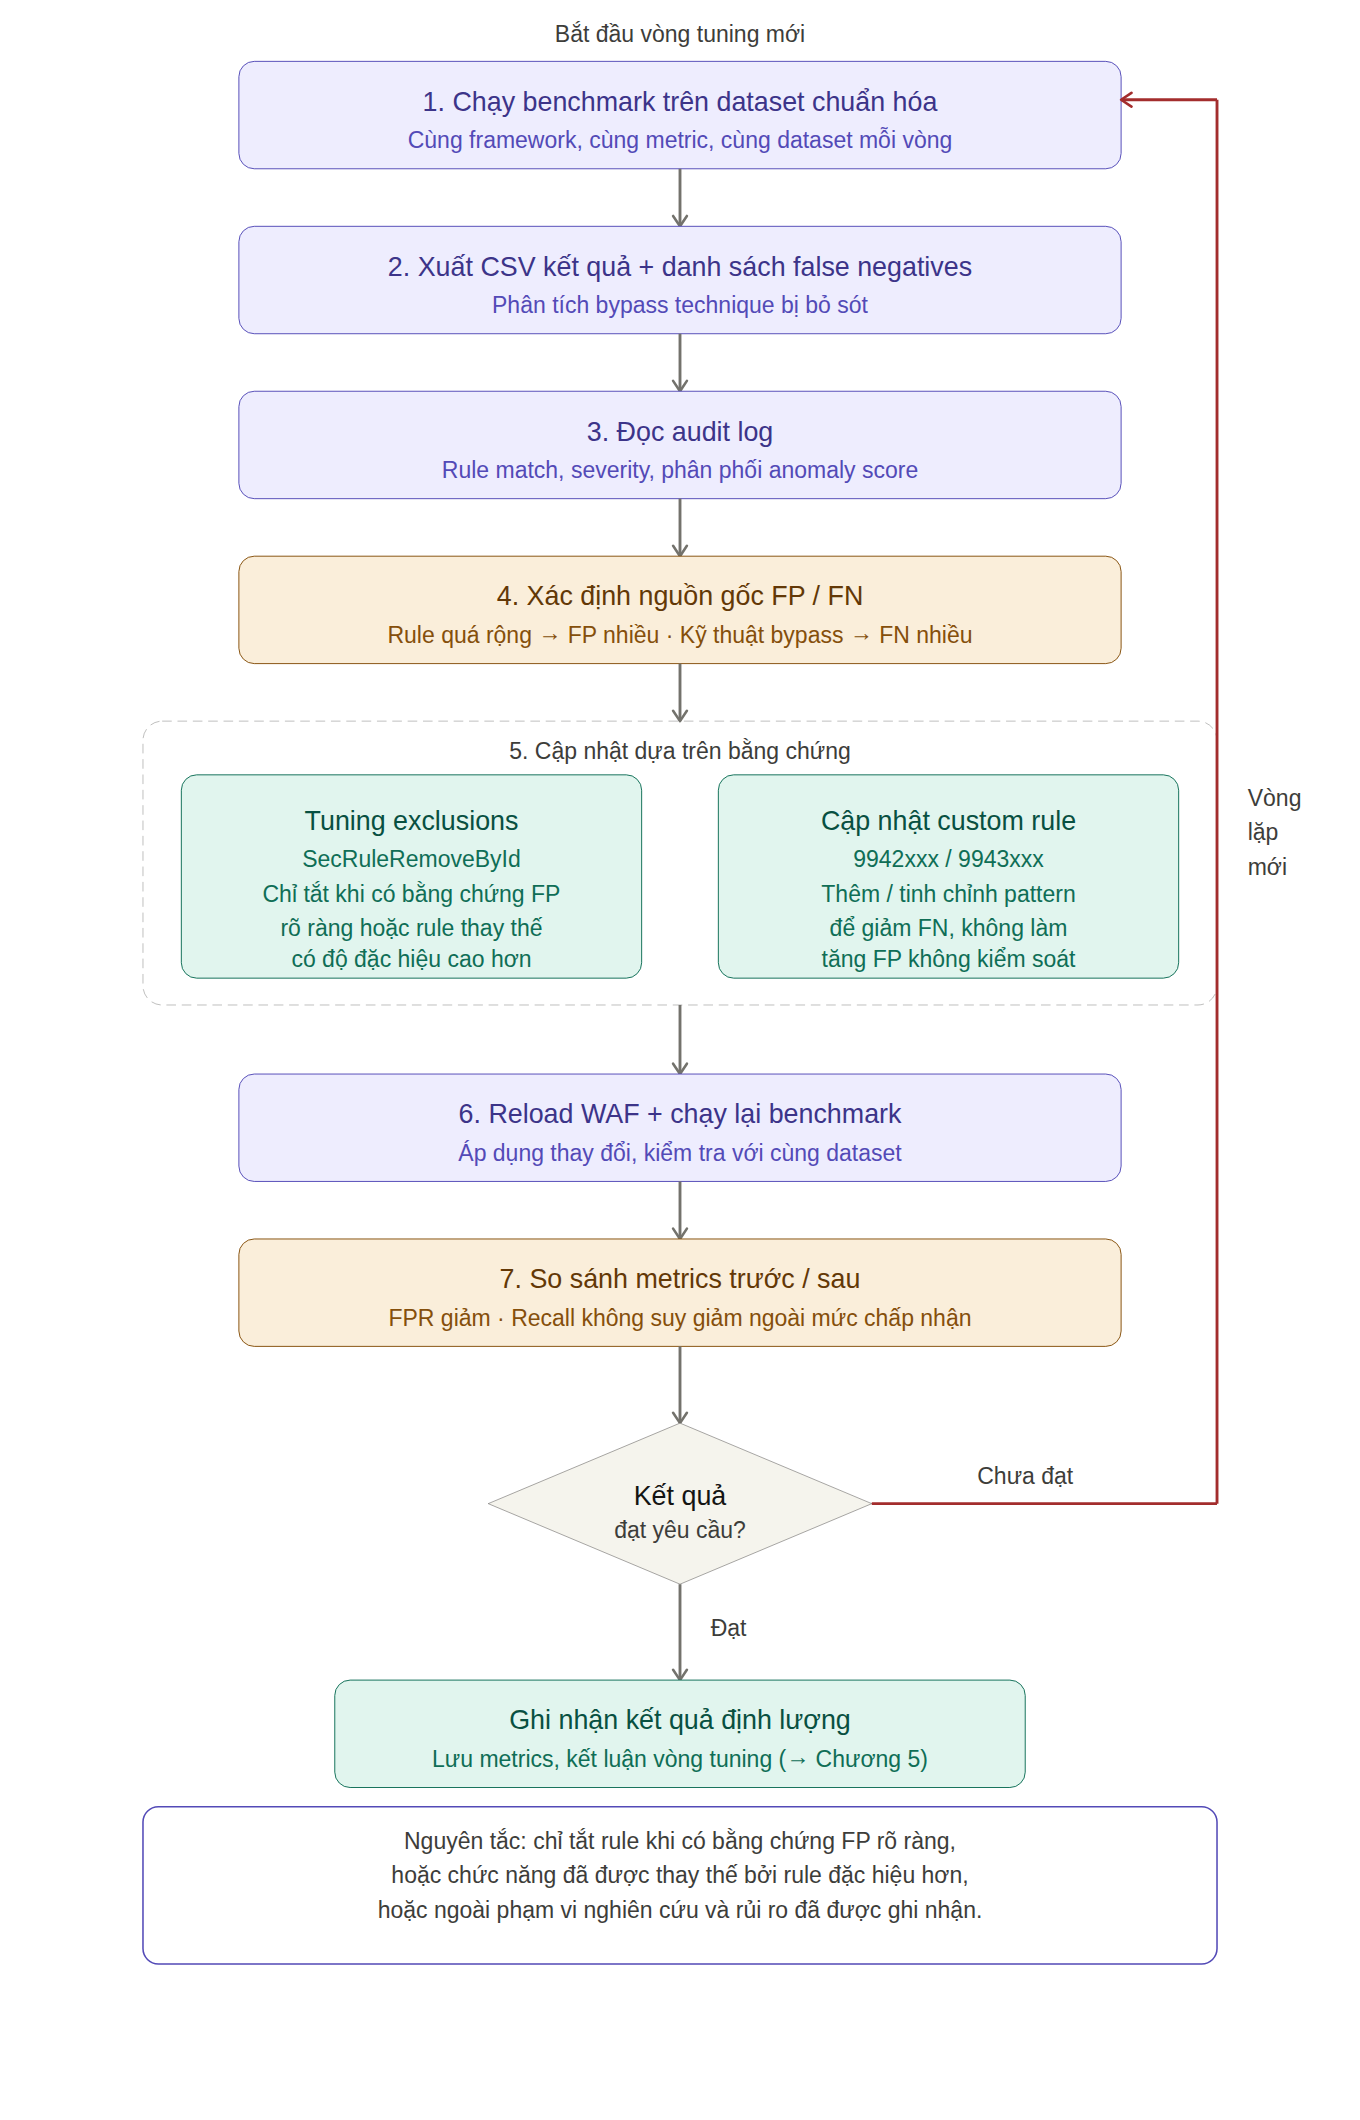
\includegraphics[width=0.92\textwidth,height=0.80\textheight,keepaspectratio]{Chapter3/tuning_iterative_process.png}
    \caption{Quy trình tuning exclusions và cập nhật rule dựa trên dữ liệu}
    \label{fig:tuning-iterative-process}
\end{figure}

Quy trình tuning gồm các bước sau:

\begin{enumerate}
    \item Chạy benchmark trên một hoặc nhiều dataset đã chuẩn hóa.
    \item Xuất CSV kết quả và danh sách false negatives để phân tích bypass.
    \item Đọc audit log để xác định rule match, severity và phân phối anomaly score.
    \item Xác định rule gây FP nhiều hoặc nhóm kỹ thuật gây FN nhiều.
    \item Cập nhật custom rule hoặc tuning exclusions dựa trên bằng chứng.
    \item Reload môi trường WAF và chạy lại benchmark.
    \item So sánh metrics trước/sau để bảo đảm FPR giảm mà recall không suy giảm ngoài mức chấp nhận.
\end{enumerate}

Chiến lược tuning không phải là tắt CRS một cách tùy tiện. Các custom rules v2 vẫn được giữ lại; CRS scoring engine vẫn được dùng để tổng hợp điểm; chỉ một số rule phát hiện gây nhiễu được loại khỏi pipeline. Với XSS, nhiều rule CRS nhóm \path|941xxx| được loại vì logic phát hiện đã được thay thế bằng XSS v2 có context rõ hơn. Với SQLi, một số rule \path|942xxx| được loại do quá nhạy hoặc trùng với semantic SQLi rules. Ngoài ra, một số rule protocol/character và RCE/Shell cũng được loại trong môi trường benchmark vì chúng nằm ngoài phạm vi chính XSS/SQLi hoặc tạo FP trên ký tự hợp lệ.

Bảng~\ref{tab:tuning-exclusions-groups} tóm tắt các nhóm exclusions quan trọng.

{\small
\renewcommand{\arraystretch}{1.2}
\begin{longtable}{|L{0.20\textwidth}|L{0.22\textwidth}|L{0.30\textwidth}|L{0.18\textwidth}|}
\caption{Các nhóm rule được tuning bằng SecRuleRemoveById}\label{tab:tuning-exclusions-groups}\\
\hline
\textbf{Nhóm rule} & \textbf{Ví dụ ID} & \textbf{Lý do thiết kế} & \textbf{Rủi ro/ghi chú} \\
\hline
\endfirsthead

\hline
\textbf{Nhóm rule} & \textbf{Ví dụ ID} & \textbf{Lý do thiết kế} & \textbf{Rủi ro/ghi chú} \\
\hline
\endhead

XSS CRS & \path|941100|, \path|941160|, \path|941390| & Giảm FP từ các rule XSS tổng quát, tránh trùng logic với XSS v2. & Cần bảo đảm XSS v2 cover đủ nhóm tấn công trong phạm vi. \\
\hline
SQLi CRS & \path|942100|, \path|942131|, \path|942370| & Giảm FP từ libinjection, character anomaly và rule SQLi quá rộng. & Tắt \path|942100| là trade-off vì mất một heuristic rộng. \\
\hline
Protocol/character & \path|920230|, \path|920272|, \path|920273| & Một số rule quá nghiêm với traffic benchmark hoặc input encoded hợp lệ. & Cần đánh giá lại nếu triển khai production. \\
\hline
RCE/Shell & \path|932120|, \path|932130|, \path|932231| & Giảm FP trên ký tự shell-like và nội dung ngoài phạm vi XSS/SQLi. & Rủi ro trung bình vì giảm coverage ngoài phạm vi đề tài. \\
\hline
Nhóm khác & \path|933161|, \path|934101| và một số rule lẻ & Loại bỏ các nguồn FP phát hiện qua audit log và benchmark. & Cần ghi nhận lý do tuning theo từng môi trường. \\
\hline
\end{longtable}
}

Cần nhấn mạnh rằng tuning exclusions là cấu hình phục vụ nghiên cứu và benchmark cho phạm vi XSS/SQLi. Nếu áp dụng trong production, người vận hành cần đánh giá lại theo traffic thật, loại ứng dụng, rủi ro cần bảo vệ và yêu cầu compliance. Đặc biệt, nhóm RCE/Shell và một số heuristic rộng của CRS không nên bị tắt mặc định nếu hệ thống cần bảo vệ toàn diện hơn ngoài XSS và SQLi.

Phần thiết kế tuning này là cơ sở kỹ thuật để trả lời RQ4 ở chương đánh giá. Kết luận về tuning không thể chỉ dựa trên việc số FP giảm, mà phải kiểm tra đồng thời FPR, recall và nhóm rule bị vô hiệu hóa để thấy rõ trade-off bảo mật.

\section{Khả năng bảo trì và giới hạn của giải pháp}
\label{sec:solution-maintainability-limitations}

Một hạn chế lớn của rule enumeration-based là regex dễ trở nên dài, khó đọc và khó kiểm thử khi danh sách payload tăng lên. Giải pháp v2 khắc phục bằng cách tổ chức rule theo namespace và layer rõ ràng. Dải \path|9942xxx| được dành cho XSS, dải \path|9943xxx| được dành cho SQLi. Trong mỗi dải, các rule được nhóm theo kỹ thuật: core, structural, encoded, DOM, advanced đối với XSS; classic, blind, error/OOB, advanced và heuristic đối với SQLi.

Cách tổ chức này giúp quá trình bảo trì có quy trình rõ hơn. Khi xuất hiện một bypass mới, người phát triển không cần thêm payload vào một regex lớn. Thay vào đó, có thể phân loại bypass thuộc nhóm nào: encoding, DOM context, protocol URI, time-based blind, comment obfuscation hay schema enumeration. Sau đó rule mới được thêm vào lớp tương ứng hoặc rule hiện có được chỉnh sửa có kiểm soát. Việc benchmark lại sau thay đổi giúp kiểm tra tác động tới cả recall và FPR.

Message, tag, severity và rule ID cũng hỗ trợ phân tích audit log. Khi request bị chặn, người vận hành có thể biết rule nào khớp, thuộc lớp nào, severity bao nhiêu và đóng góp điểm như thế nào vào anomaly score. Điều này giúp giải pháp dễ giải thích hơn so với mô hình AI black-box hoặc regex monolithic không có phân tách kỹ thuật rõ ràng.

Tuy nhiên, giải pháp vẫn có giới hạn. Custom rules v2 không thay thế hoàn toàn OWASP CRS, không tuyên bố phát hiện mọi biến thể XSS/SQLi trong tương lai và có thể vẫn tạo false positives trong các ứng dụng hợp lệ có chứa HTML, JavaScript hoặc SQL snippets. Base64 decode cũng cần được áp dụng cẩn trọng vì nhiều ứng dụng hợp lệ có thể truyền dữ liệu Base64 như ảnh, token hoặc blob dữ liệu. Cuối cùng, tuning exclusions trong môi trường benchmark không phải cấu hình production mặc định; các exclusions cần được xem xét lại theo yêu cầu bảo vệ của hệ thống thực tế.

Các nguyên tắc bảo trì này liên hệ trực tiếp với RQ1 và RQ3: nếu rule được tổ chức theo execution context và semantic pattern, việc mở rộng coverage không cần quay lại cách liệt kê payload đơn lẻ. Chúng cũng tạo cơ sở để thảo luận RQ5, vì khả năng giải thích bằng rule ID, message và severity là một ưu điểm quan trọng của WAF rule-based so với mô hình AI black-box.

\section{Tổng kết chương}
\label{sec:chapter3-summary}

Chương này đã trình bày phương pháp nghiên cứu và giải pháp đề xuất cho bài toán tối ưu bộ luật WAF. Quy trình nghiên cứu được tổ chức theo hướng lặp, bắt đầu từ phân tích CRS/rule gốc, thiết kế generalized rules, phân tích FN/FP và tuning dựa trên dữ liệu. Giải pháp được xây dựng trên ModSecurity/OWASP CRS, bổ sung hai nhóm custom generalized rules v2: XSS trong dải \path|9942xxx| và SQLi trong dải \path|9943xxx|.

Chương cũng đã trình bày decode pipeline trong luật phát hiện, cách rule v2 tích hợp với anomaly scoring của CRS, chiến lược tuning exclusions, khả năng bảo trì và các giới hạn của giải pháp. Chương tiếp theo sẽ trình bày thiết kế thực nghiệm và phương pháp đánh giá dùng để kiểm chứng các thành phần giải pháp vừa nêu.
